\subsection{Time, Length, and Lorentz Transformations} 

(Answers to M\Alph{subsection} problems are on page \pageref{lorentz_prob_answers}.)

\begin{Exercise}
In class, we imagined an experiment in which Anna held out her arms with a lightbulb in each hand, and turned on the lightbulbs simultaneously.  Take each of Anna's arms to be one meter long.
\begin{enumerate}[nosep,label=(\alph*)] 
\item Draw a spacetime diagram (or ``Minkowski diagram'') in the reference frame of Anna showing three events: each of the two lightbulbs turning on, and the photons from both bulbs arriving at the tip of Anna's nose.  Take the photons arriving at Anna's nose to occur at $x=0$ and $t=0$.  (Yes, this means that the photons were emitted at some time $t<0$.) 
\item Anna turns on the bulbs in a train car moving at speed $v=0.5c$ in the positive $x$ direction relative to Bob, who is standing beside the tracks.  What is Bob's velocity relative to Anna?  (Be careful with your signs here!).  
\item Bob's nose is exactly even with Anna's nose at $t=t'=0$ and $x=x'=0$, so the third event (photons arriving at Anna's nose) happens at $x'=0$ and $t'=0$.  Use the Galilean transformations to find the coordinates of the other two events in Bob's reference frame.  
\item Draw another spacetime diagram showing those same three events in the reference frame of Bob, according to the Galilean transformations you used in part (c).  
\item According to your work in the previous two parts, what are the speeds of the photons from the two lights in Bob's reference frame? 
\end{enumerate} 
(Note: the velocities you find in part (e) are different from the speed of light $c$, which violates the postulate of relativity.  The purpose of this exercise is to point out that the Galilean transformations are simply not correct at high speeds, for precisely this reason.)
\end{Exercise}
\begin{Answer}
(b) $v=-0.5c$ (e) $1.5c$ and $0.5c$.  
\end{Answer}

\begin{Exercise}
In  Lab~\ref{time_dilation_lab}, we imagined Anna in a train car, moving fast enough that her clock and Bob's clock differed by a factor of 1.5.  Exactly how fast would Anna have to be going for that to happen? 
\end{Exercise}
\begin{Answer}
MC3. $0.745c$
\end{Answer}


\begin{Exercise}
Anna is traveling on a spacecraft at a speed of $0.8c$ relative to the Earth, and is taking advantage of her travel time by working on her physics homework.  According to Anna, it took her one hour to finish her homework.  (a)~How long does it take Anna to finish her homework according to Bob, who is sitting at his desk in Richmond? (b)~From what we did in class, you know that for a problem like this, the times according to Anna and Bob will always differ by a factor of $\gamma$.  The trick is to figure out whether to multiply or divide by $\gamma$; that is, to determine who measures the shorter time and who measures the longer time.  Now that you have checked your answer to part (a) below, how do you know for sure whether Anna or Bob measures the shorter time?  (Hint: what are the two events you are finding $\Delta t$ for, and how do you determine who measures the proper time between those two events?)
\label{anna_bob_hw1}
\end{Exercise}
\begin{Answer}
(a) 1 hour and 40 minutes
\end{Answer}


\begin{Exercise}
A GPS satellite orbits the Earth at a speed of $14,000$~km/hr.  The GPS satellite carries a very accurate atomic clock on board, which can measure time very precisely.  If the clock on a satellite starts out synchronized to a clock on the surface of the Earth, by how much will the clock on Earth differ from the clock on the satellite after one full day, based on the velocity of the satellite?  To do this calculation, you will need to use a calculator that can keep a LOT of digits; the default calculator in Windows will work fine, for instance.  (Also note: I have to say ``based on the velocity of the satellite'' because there's also an additional gravitational effect due to the altitude of the satellite, which is about five times larger than what you're calculating here.) 
\end{Exercise}
\begin{Answer}
About 7 microseconds
\end{Answer}


\begin{Exercise}
Anna travels at speed $0.7c$ by spacecraft to the nearby star Proxima Centauri, which is a distance of 4.2~light-years away from Earth in the Earth's reference frame.  (a)~How long will the trip take her in the Earth's reference frame?  (b)~By how much will Anna age during her trip?  That is, how long does the trip take in Anna's reference frame?  (c)~How far is Proxima Centauri from Earth in Anna's reference frame?  (Hint: if you laid a 4.2~light-year-long ruler between the two stars, how long would the ruler be in Anna's frame?)  (d)~Bob, on Earth, calculates Anna's speed by dividing the distance she travels by the time of her trip, in his reference frame.  Anna calculates her speed by dividing the distance she travels by the time of her trip, in her own reference frame.  What do Anna and Bob each calculate for Anna's speed, and do they agree?
\end{Exercise}
\begin{Answer}
(a) 6 years (b) 4.29 years (c) 3 light-years (d) Both had better calculate $0.7c$.
\end{Answer}


\begin{Exercise}
Anna and Bob perform another experiment with a flashlight and a mirror, similar to what they did in Activity~1 of Lab~\ref{time_dilation_lab}.  This time, Anna rides the train in the $+x$ direction with velocity $v=+0.75c$.  Bob holds the flashlight at the origin, 1~m above the mirror, turning it on at time $t=t'=0$ in both of their frames.  (a)~Draw Minkowski diagrams for the photon in both Anna's and Bob's reference frames, under the (incorrect) Galilean Transformations.  Be careful with your signs! (b)~Draw Minkowski diagrams for the photon in both reference frames under the (correct) Lorentz Transformations.  (c)~Using the Mathematica applet, estimate the coordinates $(x', ct')$ when the particle is detected according to Anna in part (b).  (d)~Calculate the exact value of $c \Delta t$ (in meters) according to both Anna and Bob, where $\Delta t$ is the time between the emission and detection of the photon.  (Hint: one of them measures the proper time $\Delta t_0$.) 
\end{Exercise}
\begin{Answer}
(d) Bob measures $c \Delta t=2$~m.  Anna measures $c \Delta t=3.02$~m.  Incidentally, if you would like to check your other answers with me for parts (a) through (c), I'll be happy to do that during office hours.  I often don't post answers here for qualitative questions (like graphs, or yes/no or multiple choice questions), because once you see those answers, even by accident, it's too easy to convince yourself that of course you knew how to get that answer on your own when you really didn't.  But once you've given the problem a try, I'm always happy to chat with you about whether you got it right.
\end{Answer}


\begin{Exercise}
In reference frame $S$, an event occurs at coordinates $x=2$ m, $t=4~{\rm m}/c$.  Find the coordinates $(x',t')$ of this event in a reference frame $S'$ moving with respect to $S$ at $v=-0.6c$.
\end{Exercise}
\begin{Answer}
$x'=5.5$~m, $t'=6.5~{\rm m}/c$
\end{Answer}


\begin{Exercise}
Anna is riding on a train at velocity $v=+0.6c$.  Bob stands on the ground beside the tracks.  He snaps his fingers at position $x=4$~m, at time $t=8$~m/$c$.  Where and when does the snap occur in Anna's reference frame?  (Although the problem doesn't say it explicitly, you can always assume that Anna's and Bob's origins coincide at $t=t'=0$.)
\end{Exercise}
\begin{Answer}
MC9. $x'=-1$ m, $ t'=7$ m/$c$
\end{Answer}


\begin{Exercise}
In problem \ref{anna_bob_hw1}, Anna traveled on a spacecraft at a speed of $0.8c$ relative to the Earth.  According to Anna, it took her one hour to finish her physics homework.  You should have found that according to Bob (on Earth), Anna finished her homework in 1 hour and 40 minutes.  We didn't mention that Bob was also doing his physics homework that day, and according to Bob it took him 1 hour to finish it.  How long does it take Bob to finish his homework according to Anna?
\end{Exercise}
\begin{Answer}
MC11. Also 1 hour and 40 minutes.  (If you calculated 36 minutes, then you may want to review 
Problem~\ref{federation_and_romulans_prob}.  When two spacecraft pass each other at speed $v$, it's meaningless to try to discern which one is really moving and which one is standing still; both reference frames are equally valid.  That's true for any two reference frames, even when one is based on a tiny spaceship and one is based on a planet.  Bob's planet is doubtless more spacious than Anna's spacecraft, but their two reference frames are nevertheless equally valid.)
\end{Answer}

[Note: problems \ref{first_lorentz_derivation_prob} through \ref{fourth_lorentz_derivation_prob} below relate directly to the video on Blackboard in which I derive the Lorentz transformations, and the four pages of notes that go along with them.]  

\begin{Exercise}
\label{first_lorentz_derivation_prob}
In the first page of the notes, I reason that the Lorentz transformations must be linear in $x$ and $t$, that is, $x'=Ax+Bt$.  Write one or two sentences explaining in words how we know that this must be true.
\end{Exercise}

\begin{Exercise}
On the second page of notes, I imagine two special cases of an object that starts at the origin at time $t=0$.  For each of these special cases, write briefly in words what the two situations are, and draw Minkowski diagrams with worldlines for the object, one in frame $S$, one in frame $S'$.  (I'm asking for two descriptions and four Minkowski diagrams in total.)
\end{Exercise}

\begin{Exercise}
At the bottom of the second page of notes, I made an algebra error in deriving Equation~4.  Find the mistake, and write Equation~4 correctly.
\end{Exercise}

\begin{Exercise}
\label{fourth_lorentz_derivation_prob}
At the top of page 3, and again at the top of page 4, I use a ``trick'' in which I rewrite a transformation equation after switching which frame I call $S$ and which frame I call $S'$.  What two things do we have to change in a transformation equation to account for this switch in the labeling of the two reference frames?  (Hint: primes and a sign.)
\end{Exercise}

\begin{Exercise}
In class, I gave a short justification of why the Lorentz transformations require that $y'=y$ and $z'=z$.  The example I used involved Anna on a train, just barely making it under a low-clearance bridge.  Think of another good example to use to motivate why this must be true, and describe it here briefly.  (Maybe two objects moving towards each other?  Maybe something in sports---ooh, I bet either baseball or archery could work well!  Remember, the motion of your two objects is along the $x$ direction, so you can focus your argument on either the $y$ or $z$ axis; your example doesn't have to focus on height.)
\end{Exercise}


\begin{Exercise}[difficulty=0]
A tortoise (top speed $0.25c$) and a hare (top speed $0.5c$) are having a race.  They have agreed on a straight-line course that is 2~light-seconds long (its proper length).  A zebra agrees to officiate.  The Minkowski diagram on the right shows what happens when a starting gun sounds, as observed in the Earth reference frame:

\begin{minipage}{0.70 \textwidth}
\begin{itemize}[nosep]
\item The tortoise, hare, zebra, and all spectators synchronize their watches to $t=0$.
\item The tortoise accelerates nearly instantaneously to his top speed of $0.25c$, which he maintains through the end of the race.  
\item The zebra accelerates nearly instantaneously to $0.5c$, and stops nearly instantaneously right at the finish line to observe the end of the race.  
\item The hare hot-dogs around at the starting line, mugging to cameras and waving to fans for a full four seconds.  Only then does he accelerate nearly instantaneously to his top speed of $0.5c$, which he maintains through the end of the race.  
\end{itemize}

\end{minipage}
\begin{minipage}{0.29 \textwidth}
\hspace{\fill}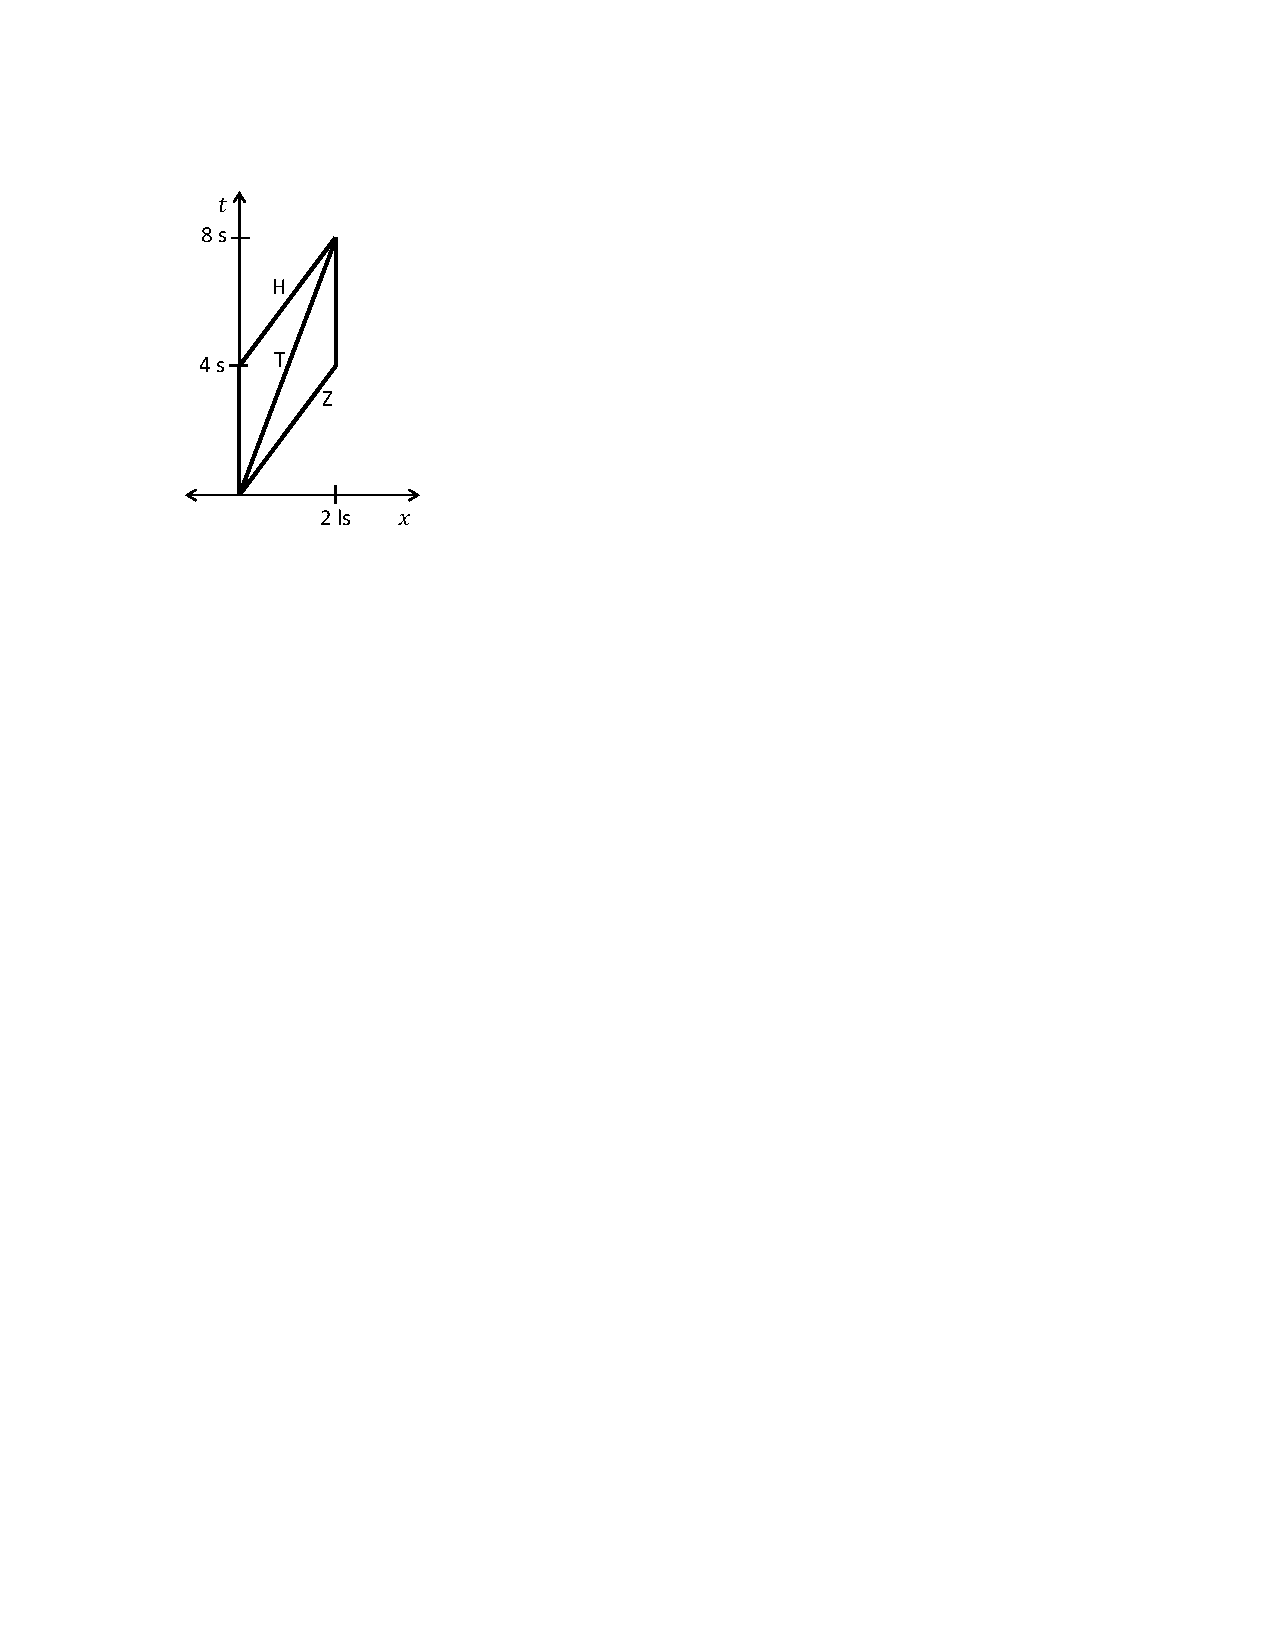
\includegraphics[scale=0.85]{M_problems/velocities_causality/tortoise_hare.pdf}

\end{minipage}

\begin{enumerate}[nosep,label=(\alph*)]
\item Draw a qualitative Minkowski diagram of the race in the reference frame of the tortoise.
\item How much time passes on the tortoise's wrist watch while he is running the race?
\item In the tortoise's reference frame, at what time does the zebra stop running, and at what time does the hare start running?  
\item According to the hare's wrist watch, how long does it take the hare to complete the course?  (The total time, including the time he was just standing around showboating.)
\item In the reference frame of the tortoise, what is the speed of the hare, once he starts running?
\end{enumerate}
At the end of the race, the zebra declares the race to be a tie.  The tortoise and hare each stare at their watches in amazement.  The other animals all boo and throw trash onto the field.  
\begin{enumerate}[resume*]
\item Do the tortoise, the hare, and the spectators agree or disagree about who crossed the finish line first?  Explain.
\item What do the tortoise, the hare, and the spectators measure for the time it took each competitor to complete the course?  (That's six times to compare.)  Do they agree or disagree about which competitor had the shortest time?  Again, explain.
\end{enumerate}
\end{Exercise}
\begin{Answer}
(b) 7.75 s (c) 3.61 s; 4.13 s (d) 7.48 s (e) $0.286c$ (f) They agree.  (g) As a check for your results, the sum of all six times is 46.46 seconds.  In fact, though their numbers differ, the tortoise, the hare, and all the other animals all agree on the ultimate outcome of the race, by any reasonable measure.  (The other animals only booed and threw trash on the field because they got caught up in the moment and it seemed like the right thing to do.)
\end{Answer}

\begin{Exercise}[difficulty=0]
Suppose you drive for 2 hours at 70 mph up to Washington DC, and then return back to Richmond at the same speed.  Due to time dilation, what is the difference between how much you aged, and how much your friend aged who stayed in Richmond? In answering this question, please do the calculation using a binomial series expansion for gamma, as in Lab~\ref{binomial_expansion_lab}.

\end{Exercise}
\begin{Answer}
The difference is 78 picoseconds.
\end{Answer}


\bigskip\bigskip
\pagebreak[3]
\textbf{Answers to Selected {\thesubsection} Problems:}
\label{lorentz_prob_answers}
%\shipoutExercise
\shipoutAnswer

\cleardoublepage
